% $Id%

\hypertarget{appendix-start}{}\label{s:appendix-start}
% \addcontentsline{toc}{section}{Anhang} 
% \addcontentsline macht nur Eintrag ins Inhaltsverzeichnis und deren PDF-Darstellung im linken Frame (mit den Kapitel�berschriften). 

%be_2005: Arbeitet man hier mit \addcontentsline{toc}{section}{Anhang} und man
%         nutzt statt \section das \subsection, damit es korrekterweise
%         unterhalb von Appendix einetragen wird, hat es das Pr�fix ".1" oder ".2"
%         statt "A" oder "B".
% --> L�sung: nur section (da der Link im Content vorher immer eine Seite zu fr�h ansprang)

\section{Anhang}

% be_2005: - Mit ref (zu label) kann man eine anspringbare Kapitel-NUMMER einf�gen.
%          - Mit hyperlink (zu hypertarget) einen anspringbaren Titel (den man aber
%            selbst nochmal angeben muss).
%          - Aber wie kann man gleich den Titel selbst als Referenz erhalten ??? 
\hyperlink{appendix-menutree}{(Anhang A: CrypTool Men"ubaum)}

\hyperlink{appendix-authors}{(Anhang B: CrypTool-Skript-Autoren)}

\hyperlink{appendix-movies}{(Anhang C: Filme und Literatur mit Bezug zur Kryptographie)} 




\newpage
\enlargethispage{1cm}
\subsection{CrypTool-Men"us}
\hypertarget{appendix-menutree}{}\label{s:appendix-menutree}

Dieser Anhang enth"alt den kompletten Men"u-Baum der CrypTool\index{CrypTool}-Version 1.3.10.

Welche Men"ueintr"age gerade aktiv (also nicht ausgegraut) sind, 
wird durch den Typ des aktiven Dokumentenfenster bestimmt.
So ist z.~B.  die Brute-Force Analyse\index{Angriff!Brute-force} f"ur DES 
nur verf"ugbar, wenn das aktive Fenster in Hexadezimal-Darstellung 
ge"offnet ist, w"ahrend der Men"ueintrag
"`Zufallsdaten erzeugen\dots"' immer verf"ugbar ist. 

Folgende Dokumenttypen gibt es in CrypTool:
\begin{center}
\begin{tabular}{rl}
\bf Codebuchstabe & \bf Dokumententyp \\
A & ASC\\
T & Text\\
H & Hexadezimal\\
P & Plot\\
\end{tabular}
\end{center}

\clearpage
\begin{figure}[hb]
\begin{center}
\vspace{-30pt}
%\frame{
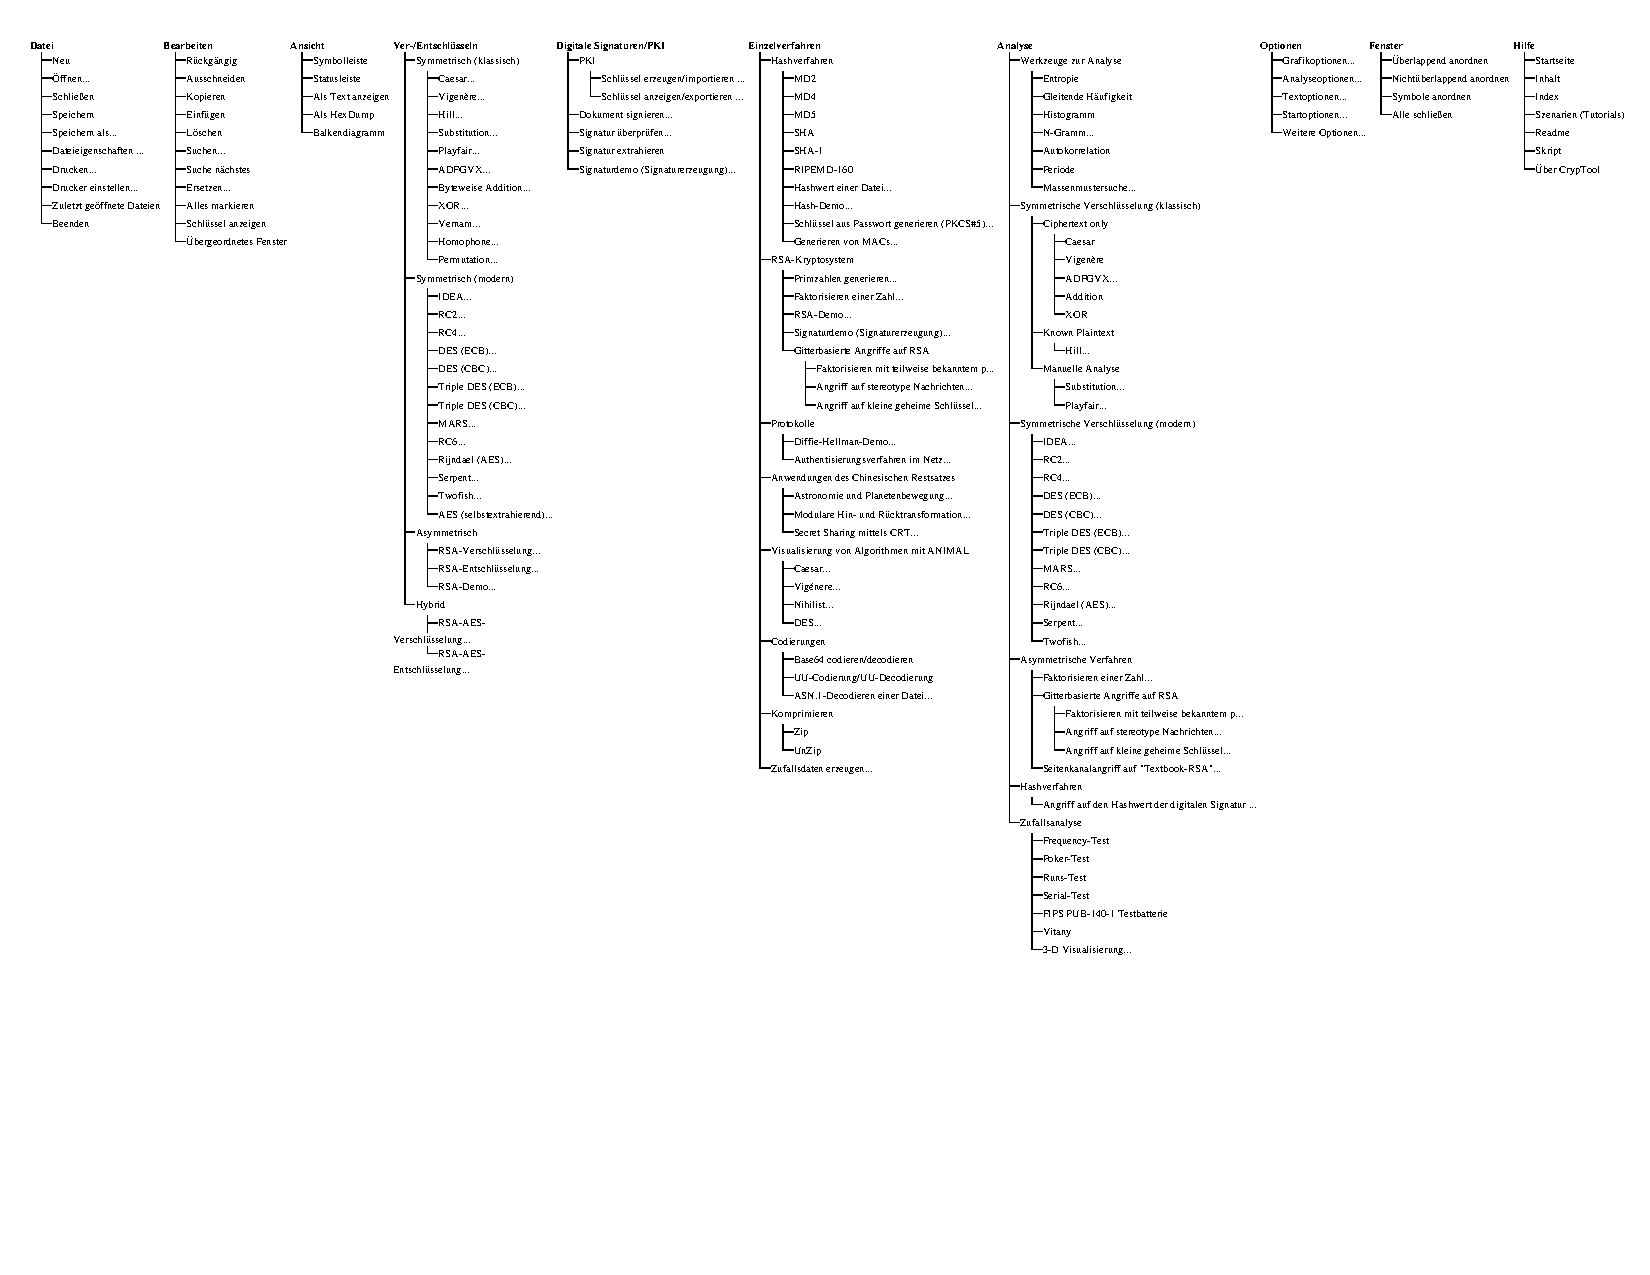
\includegraphics[scale=0.75, angle=270, viewport=14 72 835 590]{figures/cryptool-menu-de}
%viewport=rand-links? rand-unten breite hoehe? [bezogen auf querformat]
%}
\caption{Komplette "Ubersicht "uber den CrypTool-Men"u-Baum} 
\label{menuoverview}
\end{center}
\end{figure}
\clearpage

